\documentclass{article}

\usepackage{amsmath,amssymb}
\usepackage{tikz}
\usepackage{pgfplots}
\usepackage{xcolor}
\usepackage[left=2.1cm,right=3.1cm,bottom=3cm,footskip=0.75cm,headsep=0.5cm]{geometry}
\usepackage{enumerate}
\usepackage{enumitem}
\usepackage{marvosym}
\usepackage{tabularx}
\usepackage{parskip}

\usepackage{listings}
\lstdefinelanguage{JavaScript}{
	keywords={typeof, new, true, false, catch, function, return, null, catch, switch, var, if, in, while, do, else, case, break, for, of, document},
	keywordstyle=\color{lila}\bfseries,
	ndkeywords={class, export, boolean, throw, implements, import, this},
	ndkeywordstyle=\color{lila}\bfseries,
	identifierstyle=\color{blue},
	sensitive=false,
	comment=[l]{//},
	morecomment=[s]{/*}{*/},
	commentstyle=\color{lightgray}\ttfamily,
	stringstyle=\color{mygreen}\ttfamily,
	morestring=[b]',
	morestring=[b]"
}
\definecolor{lightlightgray}{rgb}{0.95,0.95,0.95}
\definecolor{lila}{rgb}{0.8,0,0.8}
\definecolor{mygray}{rgb}{0.5,0.5,0.5}
\definecolor{mygreen}{rgb}{0,0.8,0.26}
\lstdefinestyle{xml} {language=xml, morekeywords={encoding, newspaper, article, title, id, published, author, xs:schema, xmlns:xs, xs:element, name, xs:sequence, xs:element, type, xs:complexType}}
\lstdefinestyle{json}{}
\lstdefinestyle{javascript}{language=javascript}
\lstdefinestyle{html}{language=html, morekeywords={main}}
\lstset{language=XML,
	basicstyle=\ttfamily,
	keywordstyle=\color{lila},
	commentstyle=\color{lightgray},
	stringstyle=\color{mygreen}\ttfamily,
	backgroundcolor=\color{white},
	showstringspaces=false,
	numbers=left,
	numbersep=10pt,
	tabsize=2,
	numberstyle=\color{mygray}\ttfamily,
	identifierstyle=\color{blue},
	xleftmargin=.1\textwidth, 
	%xrightmargin=.1\textwidth,
	escapechar=§,
	%literate={\t}{{\ }}1
	breaklines=true,
	postbreak=\mbox{\space},
	literate=%
	{Ö}{{\"O}}1
	{Ä}{{\"A}}1
	{Ü}{{\"U}}1
	{ß}{{\ss}}1
	{ü}{{\"u}}1
	{ä}{{\"a}}1
	{ö}{{\"o}}1
}

\usepackage[colorlinks = true, linkcolor = blue, urlcolor  = blue, citecolor = blue, anchorcolor = blue]{hyperref}
\usepackage[utf8]{inputenc}

\renewcommand*{\arraystretch}{1.4}

\newcolumntype{L}[1]{>{\raggedright\arraybackslash}p{#1}}
\newcolumntype{R}[1]{>{\raggedleft\arraybackslash}p{#1}}
\newcolumntype{C}[1]{>{\centering\let\newline\\\arraybackslash\hspace{0pt}}m{#1}}

\newcommand{\E}{\mathbb{E}}
\DeclareMathOperator{\rk}{rk}
\DeclareMathOperator{\Var}{Var}
\DeclareMathOperator{\Cov}{Cov}

\title{\textbf{Internet and Web Applications, Übung 4}}
\author{\textsc{Henry Haustein}}
\date{}

\begin{document}
	\maketitle
	
	\section*{Aufgabe 1: Web Crawling}
	\begin{enumerate}[label=(\alph*)]
		\item \texttt{/WORLD} $\to$ \texttt{http://www.cnn.com/WORLD} \\
		\texttt{http://www.cnn.com:80} $\to$ \texttt{http://www.cnn.com} \\
		\texttt{http://www.cnn.com/1.html\#3} $\to$ \texttt{http://www.cnn.com/1.html}
		\item BFS: zuerst Breite, dann Tiefe \\
		DFS: zuerst Tiefe, dann Breite
	\end{enumerate}
	
	\section*{Aufgabe 2: TFIDF}
	\begin{enumerate}[label=(\alph*)]
		\item Anzahl aller Wörter $N_j$ im Dokument $j$
		\begin{itemize}
			\item T1: 9 Wörter
			\item T2: 9 Wörter
			\item T3: 12 Wörter
			\item T4: 3 Wörter
		\end{itemize}
		Wie oft taucht der Begriff $t$ (\textit{computer} oder \textit{science}) im Dokument $j$ auf?
		\begin{itemize}
			\item T1: $n_{t,1} = 2 \Rightarrow TF_1 = \frac{2}{9}$
			\item T2: $n_{t,2} = 3 \Rightarrow TF_2 = \frac{3}{9}$
			\item T3: $n_{t,3} = 3 \Rightarrow TF_3 = \frac{3}{12}$
			\item T4: $n_{t,4} = 1 \Rightarrow TF_4 = \frac{1}{3}$
		\end{itemize}
		$D=4$ und $D_t=4$, weil alle Dokumente den Term enthalten $\Rightarrow IDF_t = 1$ und damit
		\begin{itemize}
			\item T1: $TFIDF_t = \frac{2}{9}$
			\item T2: $TFIDF_t = \frac{3}{9}$
			\item T3: $TFIDF_t = \frac{3}{12}$
			\item T4: $TFIDF_t = \frac{1}{3}$
		\end{itemize}
		$\Rightarrow$ T2 ist das beste Dokument.
		\item Aufblähen des Scores mit sinnlosen Begriffen möglich, ohne Mehrwert zu bieten
	\end{enumerate}
	
	\section*{Aufgabe 3: PageRank}
	PageRank is a way to prioritize results of Web keyword search based on evaluation of the link structure. Invented by Google founders Brin and Page and applied as part of Google’s ranking algorithm. Simplified assumption: A hyperlink from page A to page B is a recommendation of the content of page B by the author of A $\Rightarrow$ Quality of a page is related to its in-degree (number of incoming links). Recursion: Quality of a page is related to
	\begin{itemize}
		\item its in-degree and to
		\item the quality of pages linking to it
	\end{itemize}
	\begin{center}
		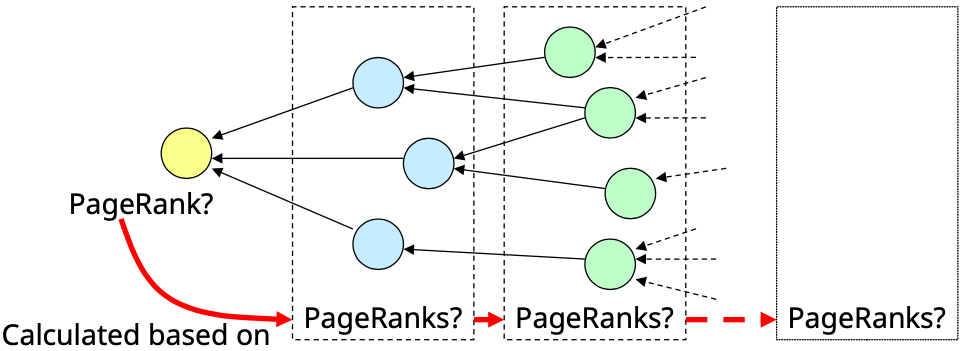
\includegraphics[scale=0.3]{pagerank}
	\end{center}

\end{document}